\documentclass{IEEEtran}
\usepackage[utf8]{inputenc}
\usepackage{acronym}
\usepackage{footnote}
\usepackage{algorithmic}
\usepackage{graphicx}
\usepackage[autostyle=true,german=quotes]{csquotes}
\usepackage{todonotes}

\usepackage{hyperref}

\long\def\comment / *#1* /{}


\begin{document}


\title{cowbus -- a small home automation bus}
\author{Robin~Backhaus \and Patrick~Kanzler \and Josef~Schnurrer \and Michael~Zapf}
\date{\today}



\maketitle

\begin{abstract}
    TODO
\end{abstract}


\section{Einleitung}

    \enquote{Smart Home} ist ein Schlagwort, um das man im 21. Jahrhundert
    kaum noch herum kommt. Der moderne Mensch möchte sein Zuhause vernetzen.
    Lichtschalter sind nicht mehr nur noch passive Komponenten in einer
    Elektroinstallation, sie sind aktive Kommunikationspartner in einem großen Netz.
    Das Licht wird nicht nur am Schalter, sondern bequem von der Couch aus mit dem
    Smartphone, automatisch durch Sensoren oder zu einer bestimmten Uhrzeit geschalt. 
    Eingehende E-Mails erscheinen nebenbei im Fernsehbild, die Verdunklung fährt 
    automatisch herunter sobald die Sonne blendet --
    all das ist keine Science Fiction mehr sondern längst Realität.

\section{Motivaton}

    Die meißten erhältlichen \enquote{Smart Home}-Lösungen sind teuer und nicht offen.
    Da die Beliebtheit solcher Systeme immer größer wird, wäre eine größere 
    Zugänglichkeit durch günstige Alternativen und langfristige Sicherheit, 
    sowie mehr Kontrolle für und durch den Anwender wünschenswert.
    Unser Fokus liegt daher auf modernen, offenen Standards und einer drahtlosen, 
    flexiblen und damit einfach zu erweiternden Netzwerktopologie.
    Mit möglichst günstigen Komponenten sollen dabei Sensoren und Aktoren 
    mit verschiedensten Funktionen ermöglicht werden.
    Eine Anknüpfung an vorhandene IP-basierende Netze durch Gateways würde die 
    Anwendungsmöglichkeiten zusätzlich erhöhen 
    und es ermöglichen bereits bestehende und neue externe Anwendungen mit dem 
    cowbus zu verbinden.

\section{Projektidee und -ziele}

    Angefangen hat der cowbus mit der Suche nach einem Projekt für die Vorlesung 
    \enquote{DIY: Personal Fabrication} 2014/2015 von Dr.-Ing. Jürgen Eckert, durch 
    Michael Zapf und Patrick Kanzler. 
    Im Rahmen der Veranstaltung hat sich dann ein Team gebildet, um eine günstige, 
    offene Alternative zu bestehenden Heimbussystemen zu entwickeln. Das Team besteht 
    aus Michael Zapf, Patrick Kanzler, Josef Schnurrer und Robin Backhaus. 
    An zentraler Stelle des Projektes steht die Kommunikation zwischen Netzwerkknoten 
    und ein Netzwerkmodell, dass möglichst flexibel erweiterbar und verkleinerbar 
    sein soll. 
    Dazu wird ein drahtloses Mesh-Netzwerk mit dezentraler Organisation implementiert 
    und an Beispiel-Sensoren und -Aktoren getestet. 
    Als besonderes Merkmal soll das System aus einzelnen, kostengünstigen, sich 
    selbst vermaschenden Knoten bestehen.
    Die Sensoren und Aktoren sollen Ereignisse erzeugen und darauf reagieren können. 
    Optional könnte nach ersten Funktionstests der ausgewählten Hardware oder im 
    Anschluss an die erfolgreiche Implementierung eines Netzwerkes der Standart 
    \enquote{6LoWPAN} implementiert werden. 
    Um keine unbrauchbare Insellösung zu entwickeln, soll neben den Aktoren und 
    Sensoren ein Ethernet-Gateway implementiert werden. Durch dieses soll das 
    Meshnetzwerk als optionales Anwendungsbeispiel eine Verbindung zu 
    einer \enquote{OpenHAB}-Instanz aufnehmen können.

\section{Projektablauf und Meilensteine}

    \subsection{Erstes Brainstorming und Projektplanung}

        Die Wahl des Projektnamen fiel nicht leicht. Wir haben uns darauf geeinigt, dass 
        wir das Projekt DIY14BUS nennen und auch so anmelden. Nachdem wir im 
        Projektverlauf mehr über Technologie und Funktionsumfang festlegen, wollten wir 
        später einen "richtigen" Namen wählen. Die Wahl viel dann auf cowbus.

        Über die Implementierung von \enquote{6LoWPAN} waren wir uns nach einem ersten 
        Brainstorming nicht mehr sicher. Obwohl dies als moderner offener Standard 
        sehr wünschenswert war, hatten wir aufgrund der begrenzten Projektzeit Bedenken 
        zu viel Zeit zu verlieren wenn die Implementierung nicht auf Anhieb gelingen 
        sollte. Vorher ein funktionierendes Mesh-Netzwerk mit den von uns gewünschten 
        Eigenschaften zu implementieren erschien uns als wichtiger, vor allem um 
        eigene Erfahrungen zu sammeln. Wir entschieden uns dafür \enquote{6LoWPAN} 
        nicht sofort zu implementieren, sondern als Option für eine Weiterentwicklung 
        nach dem Projekt offen zu halten.

        Durch die Konkretisierung unserer Projektziele entschieden wir uns eine 
        \enquote{proof-of-work}-Herangehensweise zu wählen und als erstes unser 
        Sensor-Actor-Konzept umzusetzen. Erst im Anschluss sollte ein 
        Ethernet-Gateway folgen um den Funktionsumfang des cowbus zu erhöhen.

        Zeitlich haben wir das Projekt in Monate aufgeteilt. Für den restlichen Oktober 
        gaben wir uns Zeit uns kennen zu lernen, Informationen und Wissen über bestehende 
        und zu verwendende Technologien auszutauschen und uns in das Thema einzuarbeiten.

        November: Ausprobieren von RIOT OS und Discovery-Boards, Planung und 
        Entwurf Mesh-Netzwerk.
        Dezember: Softwareentwicklung, Funktests mit Discovery-Boards, Design Prototyp.
        Januar: Implementierung und Test am Prototypen (als Sensor und Aktor).
        Februar: Fehlerbehebung und Arbeit an optionalen Projektzielen. 
        */

    \subsection{Projektinfrastruktur, verwendete Software und Hilfsmittel}
        
        GitHub, KiCad, JLink und OpenOCD, Blog

    \subsection{Kennenlernen von RIOT OS}

        Um das Rad nicht neu zu erfinden, bietet es sich an, ein eingebettetes 
        Betriebssystem auf den Knoten einzusetzen. Relativ früh wurde uns der Tipp 
        gegeben, "RIOT OS" anzuschauen. \url{http://www.riot-os.org/} 
        \enquote{The friendly Operating System for the Internet of Things.}
        RIOT OS ist ein Betriebssystem für den Bereich embedded, welches auf das 
        Thema Internet of Things optimiert wurde. 
        Damit bietet es gegenüber Konkurrenten, wie chibiOS oder FreeRTOS den Vorteil, 
        dass einiges, wie eine saubere Netzwerkkommunikation mit Unterstützung für 
        IPv6 bereits implementiert ist. 
        Es soll 6LoWPAN zum Einsatz kommen, um auf den doch relativ schwachen 
        Knotengeräten Ressourcen zu sparen.

        TODO: Multithreading, gut portierbar (Schichtenarchitektur), Lizenz: LGPLv2, c++

    \subsection{Funkchip nrf24l01+}

        2,4 GHz (ISM-Band), bis zu 2 Mbps, handliches Modul

    \subsection{Erstes Prototyping mit Discovery Boards}



    \subsection{Erste Funkübertragung und Messung der Funkreichweite}



    \subsection{ARM Cortex M0: STM32F030C8T6}

        bis zu 48 MHz, Gehäuse LQFP48 (7x7 mm)

    \subsection{Platinendesign}

        RGB-LED, Batterie-/Akkubetrieb oder USB, drei Taster, Board ca 4 cm Radius

    \subsection{Zwischenpresentation}
    

\section{Verwendete Programmiersprachen und Techniken}


\section{Aufgetretene Hindernisse und Risiken}

\section{Systemaufbau}
    TODO

    \subsection{Funkmedium}
        Als Übertragungsmedium kommt eine $2,4GHz$-Technologie
        zum Einsatz. Eine Funktechnologie eignet sich besonders gut dazu
        bereits bestehende Installationen um intelligente Komponenten
        zu erweitern, ohne größere bauliche Änderungen vornehmen zu müssen.

        Die Wahl eines ISM-Frequenzbandes (\enquote{Industrial, Scientific and Medical Band})
        ist in erster Linie bedingt durch die gute Verfügbarkeit von günstigen
        Systemkomponenten und der weltweiten Einsetzbarkeit ohne Anpassung der
        genutzten Frequenzen.

        Genutzt wird der Funkkanal im Moment als Broadcastmedium.
        Jeder Knoten kann also prinzipiell jedes Paket sehen und verarbeiten.
        Dies spart für den Anfang sehr viel Logik und Routingaufwand,
        da Pakete einfach ins Netz geflutet werden können und der entsprechende
        Empfänger (wobei das durchaus mehrere Knoten sein können -- ein Schalter
        könnte beliebig viele Lampen schalten) selbst an der Adresse erkennen
        kann, dass er darauf reagieren muss.

    \subsection{Komponenten}
        Grundsätzlich besteht der cowbus aus drei Typen von Komponenten,
        die auch in Abb. \ref{fig:comp} schematisch dargestellt sind.

        \begin{figure}
            \centering
            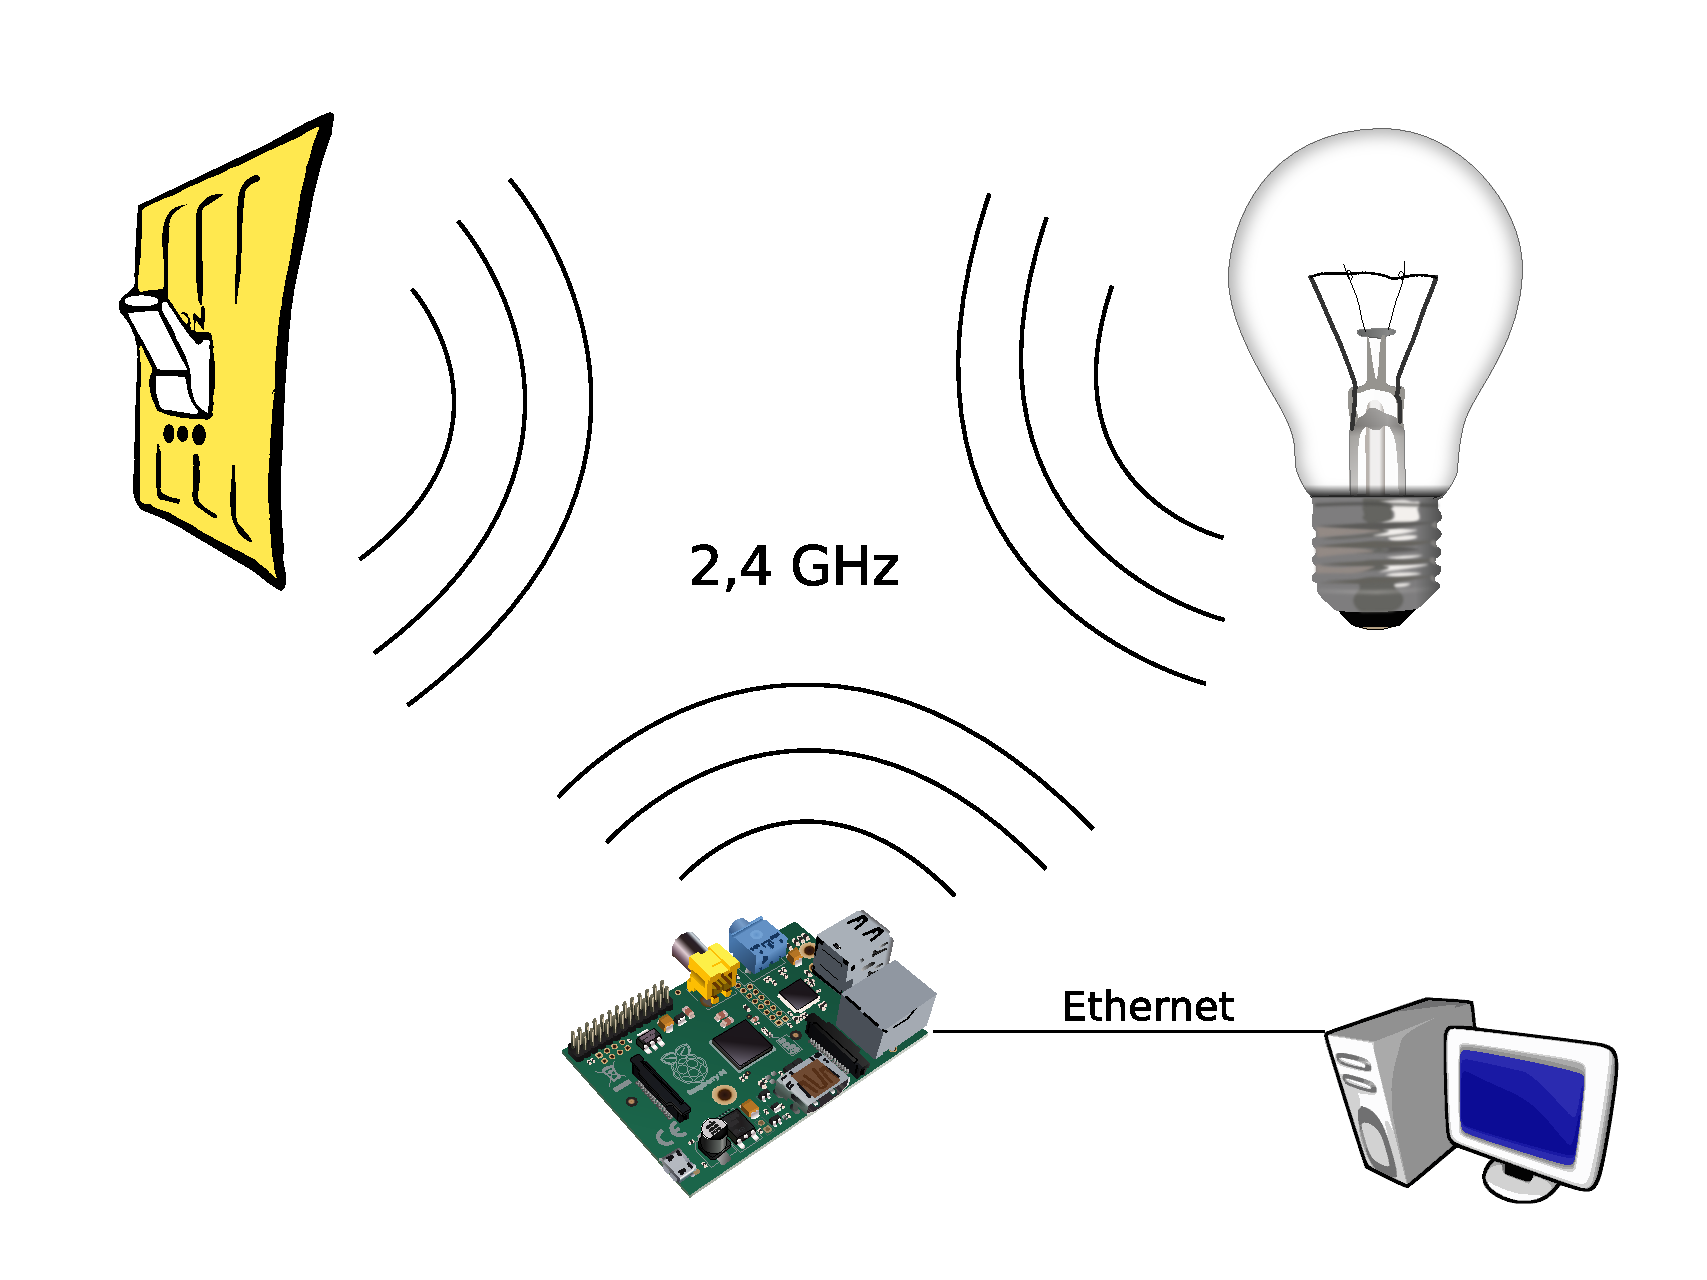
\includegraphics[width=0.5\textwidth]{img/system}
            \caption{Schematische Darstellung der beteiligten Komponententypen}
            \label{fig:comp}
        \end{figure}

        \subsubsection{Sensorknoten}\label{Sensorknoten}
            Sensorknoten sind aus Sicht des Systems im aktuellen Entwurf
            zunächst \enquote{dumm}. Sie enthalten keinerlei Wenn-Dann-Logik
            sondern produzieren ausschließlich Nachrichten mit bestimmten
            Aussagen, z.\,B. \enquote{Ich bin Knoten A und meine erste Taste
            wurde gedrückt}.
        \subsubsection{Aktorknoten}\label{Aktorknoten}
            Aktorknoten ist die eigentliche Aktion-Reaktion-Logik eingepflanzt.
            Sie lauschen auf dem Kommunikationsmedium und warten auf Anweisungen
            ihre möglichen Aktionen auszuführen.

            Dabei sind zwei Varianten vorgesehen:
            \begin{itemize}
                \item Ein Aktor kann eine Nachricht mit seiner eigenen Adresse
                    erhalten. Das bedeutet für ihn, er soll diese Aktion
                    ausführen, unabhängig davon wer das Ereignis ausgelöst hat.
                \item Ein Aktor kann programmiert werden auf bestimmte andere
                    Adressen und Nachrichten zu reagieren.
                    So kann beispielsweise eingestellt werden, dass ein Aktor
                    dann schaltet, wenn er eine Nachricht entdeckt, in der steht
                    \enquote{Ich bin Knoten A und meine erste Taste
                    wurde gedrückt} (siehe oben).
            \end{itemize}

            Durch diese zwei Varianten ist es auf der einen Seite möglich
            dezentral Nachrichten auszulösen und darauf zu reagieren, wobei
            die Auslöser, also die Sensoren selbst relativ einfach aufgebaut
            sein können. Die aufwändigere Logik, welcher Sensor welche Aktion
            auslöst, kann im Aktor implementiert werden.
            Auf der anderen Seite ist es aber trotzdem möglich, das System
            zentral zu nutzen, indem Sensornachrichten von einem zentralen
            Punkt empfangen werden, der anschließend Nachrichten mit konkreten
            Aktoradressen versendet. So können auch Aktoren \enquote{dumm}
            bleiben und können (z.B. in einem sehr kleinen, temporären Aufbau)
            ohne jede Programmierung verwendet werden, ohne dass sie von den
            konkreten Sensoren wissen müssen.

            Wie ein solches Gateway aussehen könnte zeigt der folgende Abschnitt.

        \subsubsection{Gateway (im Moment der PI)}
            Ein System, dass unabhängig von äußeren Steuerungsinfrastrukturen
            funktionieren kann, ist für die Akzeptanz im Gebäude wichtig.
            Wenn kein Lichtschalter im Haus mehr funktioniert, weil
            im Keller jemand das falsche Netzwerkkabel gezogen hat,
            wird kein Nutzer recht überzeugt sein.
            Umgekehrt ist es allerdings auch wichtig, Schnittstellen zu
            etablierten Kommunikationsstrukturen zu bieten.
            So ist eine Anbindung an vorhandene IPv4- oder IPv6-Netze
            wünschenswert, sodass auch mächtigere Komponenten integriert werden
            können, die unter Umständen noch weitere Kommunikationsmöglichkeiten
            bieten.

            Momentane Lösung dieses Wunsches ist die Integration eines Computers
            in den cowbus. Die offensichtlichste Möglichkeit war auch bei diesem
            Projekt ein Raspberry PI \footnote{\url{http://www.raspberrypi.org/}},
            der bereits alle nötigen Schnittstellen mitbringt, um direkt das
            $2,4-GHz$-Funkmodul und das vorhandene \ac{LAN} anzuschließen.

            Auf dem Raspberry PI läuft ein kleiner in C++ verfasster Daemon.
            Dieser steuert zum einen das Funkmodul und wartet auf Pakete aus
            dem Funknetz.
            Auf der anderen Seite enthält er einen kleinen Websocket-Server,
            über den von jedem beliebigen PC, der ihn über das \ac{LAN}
            erreichen kann, Pakete in das Funknetz verschickt und aus diesem
            empfangen werden kann.

            Dazu steht eine kleine HTML/JavaScript-Anwendung zur Verfügung,
            die in jedem modernen Browser läuffähig sein sollte.


    
    \subsection{Paketaufbau}
            \begin{figure}
            \centering
            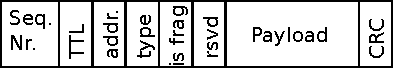
\includegraphics[width=0.5\textwidth]{img/paket}
            \caption{Aufbau der Pakete}
            \label{fig:paket}
        \end{figure}

        Hardware bedingt sind wir für die übertragenen Pakete auf 32\,Byte beschränkt, dazu in der späteren Beschreibung über den Funkchip mehr. Abbildung \label{fig:paket} zeigt den Aufbau der Pakete. Die Pakete bestehen aus:
        \begin{itemize}
            \item 5 Bit Sequenznummer: aufsteigent, für jeden Teilnehmer individuell
            \item 8-Bit Time To Live: Maximalwert, der beim Weiterleiten decrementiert wird
            \item 11-Bit Adresse: Kontexabhängig ob Sende / Empfangsadresse
            \item 4-Bit Type: Art der Nachricht
            \begin{itemize}
                \item undefined: Reservierter Typ.
                \item event: Ein Ereignis hat stattgefunden, z.B. wenn ein Taster gedrückt wurde
                \item program: Einem Aktor eine Funktion zuweisen
                \item get_name: Den Namen eines Knotens abfragen
                \item get_state: Statusabfrage
                \item get_config: Gegenstück zu program, also die Kongiguration abfragen
                \item ping: Abfrage, ob bereits ein Knoten mit angegebener Adresse vorhanden ist
                \item ping_answer: Antwort auf ping-Nachricht
                \item set_name: Den Namen eines Knotens festlegen
            \end{itemize}
            \item 1-Bit "is frag": ist das ein aufgeteiltes Paket? - Fragment Header am Anfang vom Payload
            \item 208-Bit Payload - macht 26 Byte
            \item 16-Bit CRC
        \end{itemize}
        
\section{Knoten-Prototyp-Hardware}
Tests mit den Discovery-Boards haben gezeigt, dass das Hardware-Konzept tauglich ist.
Aus diesem Grund wurde ein Protoyp entwickelt.

\subsection{Anforderungen an den Protoypen}
Ziel des cowbus ist die möglichst einfache Integration in bestehende Installationen.
Aus diesem Grund soll die fertige Platine so bemaßt sein, dass sie in einer Unterputzdose montiert werden kann.
Eine Unterputzdose ist rund und bietet etwa 4\,cm Durchmesser.

Weitere Anforderung ist, dass das Projekt erschwinglich bleibt.
In einer fertigen Installation könnte eine Vielzahl von Knoten verbaut sein, deswegen darf der Preis eines einzelnen Knotens nicht zu hoch werden.
Für die Prototypenplatine wurde ein Ziel von 20 Euro festgelegt.

Abschließend soll die Platine ausreichend sein, um alle grundlegenden Fähigkeiten des Buses zu entwickeln und abzubilden.
Das heißt sie muss sowohl die Anforderungen an einen Sensorknoten (\ref{Sensorknoten}), als auch die an einen Aktorknoten (\ref{Aktorknoten}) erfüllen.

\subsection{Umsetzung des Prototypen}


\subsubsection{Energieversorgung}
Eine der Anforderungen ist die Möglichkeit das Board in einer Unterputzdose zu montieren.
Damit gibt es zwei Möglichkeiten der Energieversorgung.
Wenn in der Dose Netzspannung verfügbar ist, kann die Energie hieraus bezogen werden.
Andernfalls muss das Board aus einer Batterie versorgt werden.

Für den Prototypen wurde die letztere Option gewählt.
Um ein Netzteil für Unterputzdosenmontage zu realisieren, müsste eine stark integrierte Baugruppe, welche bei Netzspannung arbeitet, entworfen werden.
Dies ist im Rahmen dieses Projektes nicht umsetzbar.

Aus diesem Grund wurde eine Energieversorgung per Batterie umgesetzt.
Dazu kommt der Boost-Converter TPS61221 von \emph{Texas Instruments} zum Einsatz.
Dieser zeichnet sich durch einen niedrigen Ruhestrom von $0,5 \mathrm{\mu A}$ aus.

Die Planung sah vor, die Schaltung auch optional über USB zu versorgen.
Dieser Zustand ist über Jumperstellungen auswählbar.
Das Datenblatt des Wandlers wurde dazu fehlerhaft interpretiert, da dieser nur 5V-tolerant ist.
Damit ist es in der aktuellen Hardware-Revision nicht möglich die Baugruppe über USB zu versorgen.
Als Abhilfe ist für die nächste Revision ein zusätzlicher LDO-Regler vorgesehen.

\subsubsection{Prozessor}
Die Wahl eines geeigneten Mikrocontrollers wurde früh auf 32bit-Architekturen eingeschränkt.
Am heutigen Markt ist der preisliche Unterschied nahezu irrelevant.
Zudem ist die Rechnenleistung der \enquote{größeren} Plattformen meist besser.

gewählter Chip STM32F030C8T6, genügend (ZAHL) RAM, Takt hoch, günstig, Toolchain gut.

Auch auf Discoveryboard verfügbar --> Entwicklungsstart ohne Platine

RIOT-Unterstützung

\subsubsection{Funkmodul}
* Wahl des Funkchips (hier 32-Byte Beschränkung, GFSK und Frequenzbänder/Bandbreiten)

\subsubsection{Peripherie}
Gemäß den Anforderungen ist der Prototyp mit entsprechender Peripherie bestückt.
Zum einen sind drei Taster angeschlossen, um einen grundlegenden Sensor zu modellieren.
Zum anderen befindet sich auf dem Board eine RGB-LED, welche eine primitive Form eines Aktors darstellt.

Für zukünftige Features ist ein Summer vorgesehen.
Dieser wird mit einem N-MOSFET angeschalten.
Der Summer ist dazu vorgesehen, einzelne Knoten während der Konfiguration zu erkennen.

Um Daten wie die Konfiguration des Knotens dauerhaft zu speichern, ist an den Mikrocontroller ein EEPROM über SPI angeschlossen.
Die SWD-Funktionalität des Controllers ist in Form einer Cortex-M-Debugschnittstelle herausgeführt.




    Platine, Aufbau, Designentscheidungen, ...


\section{Software und System}
    \subsection{Kommunikationsstruktur: Nachrichtenbasiert, jeder Knoten entscheidet anhand Adresse ob er interessiert ist am Inhalt}
    \subsection{RIOT - Was, Warum; evtl. auch kritische Auseinandersetzung?}


\section{Ausblick}

    \subsection{CSMA/CA}
Was geplant ist: CSMA/CA, ...;

    \subsection{Payloadkompression}
    Codierung der Zeichen in der Payload: 
    In der Payload sollen bei den Pakettypen get\_name und set\_name für den menschen lesbare Buchstaben als Name eines Knoten übertragen werden. Bei unkomprimierter Übertragung mittels Ascii Zeichen, also 8-Bit pro Zeichen, wären bei einer maximalen Payload von 208-Bit nur 26 Zeichen möglich. Zur Kompression des Knotennamens gibt es hier im Allgemeinen zwei Möglichkeiten. Zum einen können aufgrund der Buchstabenwahrscheinlichkeit in einer bestimmten Sprache ein oder mehrere Buchstaben durch Symbole ersetzt werden (z.B. mittels Huffmann oder Vektor-Huffman Codierung). Bei diesem Verfahren entstehen allerdings bei gleich langen Namen unterschiedlich lange Paylods. Da die maximale Anzahl von Buchstaben nicht mit den Buchstaben selbst variieren soll, ist dieses Verfahren ungeeignet. Die zweite Möglichkeit ist die Anzahl an möglichen Zeichen beschränken. Es sind für Namen von Knoten also nur noch Zahlen, Buchstaben und 4 Sonderzeichen (Null-Terminator, Leerzeichen, at-Zeichen, Unterstrich) zugelassen. Dies ergibt 40 Zustände pro Zeichen, die wir als gleich wahrscheinlich annehmen. Bei 40 möglichen Zuständen ergibt sich ein Informationsgehalt von $log_{2}(40) = 5,32 bit$. Für drei Zeichen ergibt sich ein Informationsgehalt von $log_{2}(40^3) = 5,32 \cdot 3 bit < 16 Bit$. Es können also 3 Zeichen in 2 Byte codiert werden. Mit 8-Bit pro Zeichen wären in der Payload 26 Zeichen möglich gewesen, mit Reduzierung der Zustände sind nun 39 Zeichen möglich.
    Anschaulich gesehen ergeben sich mit 40 Möglichkeiten pro Zeichen bei 3 Zeichen $40^3 = 64000$ Möglichkeiten. Mit 16 Bit können 65536 Zustände abgebildet werden. 
    Es werden drei ZeichenZeichen ($x_{1}$, $x_{2}$, $x_{3}$) in ein Symbol gepackt. Dieses Symbol kann durch folgendes Polynom berechnet werden:
    $$Symbol = x_{1} \cdot 40^{0} + x_{2} \cdot 40^{1} + x_{3} \cdot 40^{2}$$
    - Die Decodierung erfolgt über folgende Gleichungen:

    $$x_{1}=Symbol \% 20$$

    $$x_{2} = \frac{Symbol - x_{1}}{40} \% 40$$
    
    $$x_{3} = \frac{Symbol - (x_{1} + x_{2} \cdot 40)}{40} (\% 40)$$

    \subsection{Routing}
        
        *jeder leitet jedes Paket einmal weiter und merkt sich den Header des Paketes, damit er es kein zweites Mal weiter leitet


kritische Auseinandersetzung mit getätigten Design-Entscheidungen

\section{Zusammenfassung}



\section*{Abkürzungen}
\renewcommand{\IEEEiedlistdecl}{\IEEEsetlabelwidth{CSMA/CA}}
\begin{acronym}
    \acro{6LoWPAN}{IPv6 over Low power Wireless Personal Area Network}
    \acro{CSMA/CA}{Carrier Sense Multiple Access with Collision Avoidance}
    \acro{LAN}{Local Area Network}
    \acro{openHAB}{open Home Automation Bus}
\end{acronym}
\renewcommand{\IEEEiedlistdecl}{\relax}% remember to reset \IEEEiedlistdecl


\comment / *
\listoffigures
\clearpage

\listoftables
\clearpage
* /

\nocite*
\bibliographystyle{IEEEtran}
\bibliography{IEEEabrv,projektdoku_cowbus}

\end{document}
